% Options for packages loaded elsewhere
\PassOptionsToPackage{unicode}{hyperref}
\PassOptionsToPackage{hyphens}{url}
%
\documentclass[
]{article}
\usepackage{amsmath,amssymb}
\usepackage{lmodern}
\usepackage{iftex}
\ifPDFTeX
  \usepackage[T1]{fontenc}
  \usepackage[utf8]{inputenc}
  \usepackage{textcomp} % provide euro and other symbols
\else % if luatex or xetex
  \usepackage{unicode-math}
  \defaultfontfeatures{Scale=MatchLowercase}
  \defaultfontfeatures[\rmfamily]{Ligatures=TeX,Scale=1}
\fi
% Use upquote if available, for straight quotes in verbatim environments
\IfFileExists{upquote.sty}{\usepackage{upquote}}{}
\IfFileExists{microtype.sty}{% use microtype if available
  \usepackage[]{microtype}
  \UseMicrotypeSet[protrusion]{basicmath} % disable protrusion for tt fonts
}{}
\makeatletter
\@ifundefined{KOMAClassName}{% if non-KOMA class
  \IfFileExists{parskip.sty}{%
    \usepackage{parskip}
  }{% else
    \setlength{\parindent}{0pt}
    \setlength{\parskip}{6pt plus 2pt minus 1pt}}
}{% if KOMA class
  \KOMAoptions{parskip=half}}
\makeatother
\usepackage{xcolor}
\IfFileExists{xurl.sty}{\usepackage{xurl}}{} % add URL line breaks if available
\IfFileExists{bookmark.sty}{\usepackage{bookmark}}{\usepackage{hyperref}}
\hypersetup{
  pdftitle={A Standardized Effect Size for Evaluating and Comparing the Strength of Phylogenetic Signal},
  hidelinks,
  pdfcreator={LaTeX via pandoc}}
\urlstyle{same} % disable monospaced font for URLs
\usepackage[margin=1in]{geometry}
\usepackage{longtable,booktabs,array}
\usepackage{calc} % for calculating minipage widths
% Correct order of tables after \paragraph or \subparagraph
\usepackage{etoolbox}
\makeatletter
\patchcmd\longtable{\par}{\if@noskipsec\mbox{}\fi\par}{}{}
\makeatother
% Allow footnotes in longtable head/foot
\IfFileExists{footnotehyper.sty}{\usepackage{footnotehyper}}{\usepackage{footnote}}
\makesavenoteenv{longtable}
\usepackage{graphicx}
\makeatletter
\def\maxwidth{\ifdim\Gin@nat@width>\linewidth\linewidth\else\Gin@nat@width\fi}
\def\maxheight{\ifdim\Gin@nat@height>\textheight\textheight\else\Gin@nat@height\fi}
\makeatother
% Scale images if necessary, so that they will not overflow the page
% margins by default, and it is still possible to overwrite the defaults
% using explicit options in \includegraphics[width, height, ...]{}
\setkeys{Gin}{width=\maxwidth,height=\maxheight,keepaspectratio}
% Set default figure placement to htbp
\makeatletter
\def\fps@figure{htbp}
\makeatother
\setlength{\emergencystretch}{3em} % prevent overfull lines
\providecommand{\tightlist}{%
  \setlength{\itemsep}{0pt}\setlength{\parskip}{0pt}}
\setcounter{secnumdepth}{5}
\usepackage{setspace}\doublespacing
\usepackage{lineno}\linenumbers
\ifLuaTeX
  \usepackage{selnolig}  % disable illegal ligatures
\fi
\newlength{\cslhangindent}
\setlength{\cslhangindent}{1.5em}
\newlength{\csllabelwidth}
\setlength{\csllabelwidth}{3em}
\newenvironment{CSLReferences}[2] % #1 hanging-ident, #2 entry spacing
 {% don't indent paragraphs
  \setlength{\parindent}{0pt}
  % turn on hanging indent if param 1 is 1
  \ifodd #1 \everypar{\setlength{\hangindent}{\cslhangindent}}\ignorespaces\fi
  % set entry spacing
  \ifnum #2 > 0
  \setlength{\parskip}{#2\baselineskip}
  \fi
 }%
 {}
\usepackage{calc}
\newcommand{\CSLBlock}[1]{#1\hfill\break}
\newcommand{\CSLLeftMargin}[1]{\parbox[t]{\csllabelwidth}{#1}}
\newcommand{\CSLRightInline}[1]{\parbox[t]{\linewidth - \csllabelwidth}{#1}\break}
\newcommand{\CSLIndent}[1]{\hspace{\cslhangindent}#1}

\title{A Standardized Effect Size for Evaluating and Comparing the
Strength of Phylogenetic Signal}
\author{}
\date{\vspace{-2.5em}}

\begin{document}
\maketitle

\begin{center}
\textbf{Dean C. Adams$^{1,*}$, Erica K. Baken$^{1,2}$, and Michael L. Collyer$^2$}
\end{center}

\begin{center}11 May, 2021\end{center}

\(^{1}\)Department of Ecology, Evolution, and Organismal Biology, Iowa
State University, Ames, Iowa, USA.

\(^{2}\)Department of Science, Chatham University, Pittsburgh,
Pennsylvania, USA.

\(^{*}\)Correspondence: Dean C. Adams
\href{mailto:dcadams@iastate.edu}{\nolinkurl{dcadams@iastate.edu}}
\hfill\break

\textbf{Keywords}: comparative analysis, macroevolution \hfill\break

\textbf{Short Title}: Effect size for phylogenetic signal \hfill\break

\textbf{Research Article:}

\begin{longtable}[]{@{}rr@{}}
\toprule
words & characters \\
\midrule
\endhead
4221 & 26597 \\
\bottomrule
\end{longtable}

\textbf{Author Contributions}: DCA conceived the original idea for this
manuscript, and DCA, EKB, and MLC collaboratively developed the concept
and contributed to all portions of this manuscript. All authors approve
of the final product and are willingly accountable for any portion of
the content.\hfill\break

\textbf{Data Archiving}: Empirical data used in this paper are available
on DRYAD (associated with original articles). R-scripts for simulation
tests are found at: \url{https://github.com/deanadams/PhySigCompareZ}.
Computer code for implementing the two-sample comparison of effect sizes
is found in geomorph (\textbf{upon article acceptance}):
\url{https://cran.r-project.org/web/packages/geomorph/index.html}
\hfill\break

\textbf{Acknowledgments}: We thank E. Glynne and B. Juarez for comments
on early drafts of the manuscript. This work was sponsored in part by
National Science Foundation Grants DBI-1902511 (to DCA) and DBI-1902694
(to MLC). The authors have no known conflicts of interest.

\newpage

\setcounter{section}{0}

\hypertarget{abstract}{%
\section*{Abstract}\label{abstract}}
\addcontentsline{toc}{section}{Abstract}

\begin{enumerate}
\def\labelenumi{\arabic{enumi}.}
\item
  Macroevolutionary studies frequently characterize the phylogenetic
  signal in phenotypes, however, analytical tools for comparing the
  strength of that signal across traits remain largely underdeveloped.
\item
  In this paper, we evaluate the efficacy of Pagel's \(\lambda\) to
  correctly estimate the strength of phylogenetic signal in phenotypic
  traits across a range of input values. We find that \(\lambda\)
  behaves as a Bernoulli random variable, where estimates are
  increasingly skewed at larger and smaller input levels of phylogenetic
  signal. Further, the precision of \(\lambda\) varies with input
  signal.
\item
  Another measure, Blomberg's \emph{K}, is more consistent across a
  range of tree sizes, and exhibits a positive relationship with input
  levels of phylogenetic signal. However, that relationship is decidedly
  nonlinear. Thus, neither \(\lambda\) nor \emph{K} are suitable as
  effect sizes for measuring the strength of phylogenetic signal, and
  comparing that signal across datasets.
\item
  As an alternative, we propose a standardized effect size based on
  \emph{K}, (\(Z_K\)), which measures the strength of phylogenetic
  signal more reliably than does \(\lambda\), and places that signal on
  a common scale for statistical comparison. We develop tests based on
  \(Z_K\) to provide a mechanism for formally comparing the strength of
  phylogenetic signal across datasets, in much the same manner as effect
  sizes may be used to summarize patterns in quantitative meta-analysis.
\item
  Our approach extends the phylogenetic comparative toolkit to address
  hypotheses that compare the strength of phylogenetic signal between
  various phenotypic traits, even when those traits are found in
  different evolutionary lineages or have different units or scales.
\end{enumerate}

\newpage

\hypertarget{introduction}{%
\section{Introduction}\label{introduction}}

Investigating macroevolutionary patterns of trait variation requires a
phylogenetic perspective, because the shared ancestry of species
violates the assumption of independence among trait values that is
common for statistical tests (Felsenstein, 1985; Harvey \& Pagel, 1991).
Accounting for this evolutionary non-independence is the purview of
\emph{phylogenetic comparative methods} (PCMs): a suite of analytical
tools that condition the data by the phylogenetic relatedness of
observations (Grafen, 1989; Martins \& Hansen, 1997; Garland \& Ives,
2000; Rohlf, 2001; O'Meara, Ane, Sanderson, \& Wainwright, 2006;
Beaulieu, Jhwueng, Boettiger, \& O'Meara, 2012; Adams, 2014b; Adams \&
Collyer, 2018). PCMs are predicated on the notion that phylogenetic
signal -- the tendency for closely related species to display similar
trait values -- is present in cross-species datasets (Felsenstein, 1985;
Pagel, 1999; Blomberg, Garland, \& Ives, 2003). Indeed, under numerous
evolutionary models, phylogenetic signal is expected, as stochastic
character change along the hierarchical structure of the tree of life
generates trait covariation among taxa (Felsenstein, 1985; Blomberg et
al., 2003; Revell, Harmon, \& Collar, 2008). \hfill\break

Several analytical tools have been developed to quantify phylogenetic
signal in phenotypic datasets (Gittleman \& Kot, 1990; Abouheif, 1999;
Pagel, 1999; Blomberg et al., 2003; Klingenberg \& Gidaszewski, 2010;
Adams, 2014a), and their statistical properties -- namely type I error
rates and statistical power -- have been investigated to determine under
what conditions phylogenetic signal can be detected (Revell et al.,
2008; Revell, 2010; Boettiger, Coop, \& Ralph, 2012; Diniz-Filho,
Santos, Rangel, \& Bini, 2012; Münkemüller et al., 2012; Pavoine \&
Ricotta, 2012; Adams, 2014a; Molina-Venegas \& Rodríguez, 2017). One of
the most widely used methods for characterizing phylogenetic signal is
Pagel's \(\lambda\) (Pagel, 1999), which transforms the lengths of the
internal branches of the phylogeny to improve the fit of data to the
phylogeny via maximum likelihood (Pagel, 1999; Freckleton, Harvey, \&
Pagel, 2002). When incorporated in PGLS, \(\lambda\) serves as a tuning
parameter which is optimized via log-likelihood profiling while
evaluating the covariation between the dependent and independent
variables, given the phylogeny (Pagel, 1999; Freckleton et al., 2002).
To infer whether phylogenetic signal differs from no signal or a
Brownian motion (BM) model of evolutionary divergence, the observed
model fit using \(\hat\lambda\) may be statistically compared to that
using \(\lambda=0\) or \(\lambda=1\) via likelihood ratio tests
(Freckleton et al., 2002; Cooper, Jetz, \& Freckleton, 2010; Bose,
Ramesh, Pélissier, \& Munoz, 2019) or confidence limits (Vandelook et
al., 2019). \hfill\break

Another widely used measure is Blomberg's \emph{K} (Blomberg et al.,
2003), which characterizes phylogenetic signal as the ratio of observed
trait variation to the amount of variation expected under Brownian
motion. Blomberg's \emph{K} can be treated as a test statistic by
employing a permutation test to generate its sampling distribution
(Blomberg et al., 2003; Adams, 2014a) for determining whether
significant phylogenetic signal is present in data. Both \(\lambda\) and
\emph{K} seem intuitive to interpret, as a value of \(0\) for both
corresponds to no phylogenetic signal, while a value of \(1\)
corresponds to the amount of phylogenetic signal expected under Brownian
motion. Thus, it is tempting to regard both \(\lambda\) and \emph{K} as
descriptive statistics that measure the relative strength of
phylogenetic signal, providing an estimate of its magnitude for
comparison. \hfill\break

The appeal of Pagel's \(\lambda\) and Blomberg's \emph{K} as descriptive
statistics is that they provide a basis for interpreting ``weak'' versus
``strong'' phylogenetic signal; i.e., small versus large values of
\(\hat{\lambda}\) or \emph{K}, respectively, in a comparative sense (De
Meester, Huyghe, \& Van Damme, 2019; Pintanel, Tejedo, Ron, Llorente, \&
Merino-Viteri, 2019; Su, Villéger, \& Brosse, 2019). Nonetheless, an
important question that has yet to be considered is whether such
comparisons are analytically appropriate, and whether these statistics
are, or can be, converted to effect sizes for comparative analyses
across datasets. To be statistics representing phylogenetic signal, they
should have reliable distributional properties, which could be revealed
with simulation experiments. For instance, as a proportional random
variable bounded by \(0\) and \(1\), we might expect that
\(\hat{\lambda}\) is a random variable that follows the distribution of
a Bernoulli probability parameter (Forbes, Evans, Hastings, \& Peacock,
2011); i.e., branch lengths in a tree are scaled proportionally to the
probability that data arise from a BM process. Given a known \(\lambda\)
value used to generate random data on a tree, we would also expect that
the mean of an empirical sampling distribution of \(\hat{\lambda}\)
would approximately equal \(\lambda\); the dispersion of
\(\hat{\lambda}\) would be largest at intermediate values of
\(\lambda\), \(\hat{\lambda}\) would be predictable over the range of
\(\lambda\) with respect to tree size; the distribution of
\(\hat{\lambda}\) would be symmetric at intermediate values of
\(\lambda\) and more skewed toward values of 0 or 1; and that the
distribution of \(\hat{\lambda}\) would be more platykurtic at
intermediate values of \(\lambda\), becoming more leptokurtic toward 0
and 1 (Forbes et al., 2011). Prior work (Münkemüller et al., 2012) seems
to support some of these conjectures, based superficially on statistical
moments for a given tree size (mean, variance, skewness, and kurtosis;
see Fig. 2 of ref. (Münkemüller et al., 2012)). However, because the
``strength of Brownian motion'' was simulated as a varied
weighted-average of data simulated on trees with \(\lambda=0\) and
\(\lambda=1\) and not as prescribed values of \(\lambda\) (Münkemüller
et al., 2012), interpretation of these patterns is challenging.
\hfill\break

By contrast, for Blomberg's \emph{K}, which is positively unbounded, we
might expect that for any \(\lambda\) used to generate data, estimates
of \emph{K} might be a random variable that follows a normal
distribution, with values distributed symmetrically (Forbes et al.,
2011). This attribute seemed less reasonable based on the simulations
performed by Münkemüller et al. (2012), which suggested that
distributions were positively skewed and that Blomberg's \emph{K} might
not behave as a statistic that follows a normal distribution. However,
because their simulations used a weighted combination of simulated
phylogenetic signal strengths, strong inferences are not possible (and
distributional attributes were not the intended result of their
simulations). Thus, for both Pagel's \(\lambda\) or Blomberg's \emph{K},
evaluation of statistical moments across a range of \(\lambda\) used to
generate data would be valuable for adjudicating the reliability of
these statistics as effect sizes. Furthermore, the expected values of
these statistics appear to vary with tree size (Münkemüller et al.,
2012), making comparisons across studies challenging. Therefore,
transformation of these statistics into \(Z\)-scores would allow
evaluation of the efficacy of each statistic to yield effect sizes that
could be used for comparisons of the strength of phylogenetic signal
across traits and lineages. \hfill\break

Here we use simulation experiments to compare the distributional
attributes of \(\hat{\lambda}\) and \emph{K}, plus their effect sizes
(\(Z\)-scores), across a range of tree size and phylogenetic signal
strength. We find that estimates of \(\hat{\lambda}\) are increasingly
skewed at larger and smaller input levels of phylogenetic signal and at
smaller tree sizes, vary widely for a given input value of \(\lambda\),
and that the precision of \(\hat{\lambda}\) is not constant across its
range. By contrast, estimates of \emph{K} are more consistent across
tree sizes, and are normally distributed across the range of input
levels of \(\lambda\), making \emph{K} a more reliable statistic.
However, the relationship between \emph{K} and input levels of
phylogenetic signal is decidedly nonlinear. Thus, neither \(\lambda\)
nor \emph{K} are suitable as effect sizes for measuring the strength of
phylogenetic signal. As an alternative, we propose an effect size based
on \emph{K}, (\(Z_K\)), which provides consistent estimates of the
strength of phylogenetic signal across tree sizes and signal strength.
Further, because \(Z_K\) places that phylogenetic signal on a common
scale, it facilitates statistical comparisons of the relative strength
of phylogenetic signal across datasets. We propose a two-sample
statistic (\(\hat{Z}_{12}\)) to accomplish this task, and show that it
displays appropriate levels of type I error and model misspecification.
An empirical example is then provided to illustrate its use.

\hypertarget{simulation-methods-and-results}{%
\section{Simulation methods and
results}\label{simulation-methods-and-results}}

Methods for characterizing phylogenetic signal were evaluated by
computer simulation. Briefly, simulations were conducted by generating
pure-birth phylogenies at each of six different tree sizes
(\(n=2^5, 2^6, \cdots, 2^{10}\)), and with differing levels of
phylogenetic signal (\(\lambda=0.0, 0.5, \cdots, 1.0\)). We generated 50
random trees for each intersection of tree size and \(\lambda\). For
each \(\lambda\) within each tree size, continuous traits were then
simulated on each phylogeny under a BM model of evolution. For each set
of 50 trees we measured the mean values of \(\hat{\lambda}\) and
\emph{K}, their standard deviation, and calculated the Shapiro-Wilk
\(W\) statistic as a departure from normality (symmetry). For the
latter, a value of \(1.0\) indicates normally distributed values, while
departures from \(1.0\) indicate skewness. Simulations were then
repeated for both balanced and pectinate trees, which yielded
qualitatively similar results (see Supporting Information). Trees
containing polytomies, and an evaluation of \(\hat{\lambda}\) from
models of linear regression and phylogenetic ANOVA, were also
investigated, and results were qualitatively similar to those reported
above (see Supporting Information). \hfill\break

\hypertarget{lambda-lambda-estimates-of-phylogenetic-signal-are-inaccurate}{%
\subsection{\texorpdfstring{Lambda (\(\lambda\)) estimates of
phylogenetic signal are
inaccurate}{Lambda (\textbackslash lambda) estimates of phylogenetic signal are inaccurate}}\label{lambda-lambda-estimates-of-phylogenetic-signal-are-inaccurate}}

Computer simulations reveal that for \(\hat{\lambda}\), the
distributional expectations of a Bernoulli variable were mostly upheld.
First, the mean value of \(\hat{\lambda}\) increases as \(\lambda\)
increases. Second, the precision in estimating \(\lambda\) varies across
the range of input values, as the standard deviation of
\(\hat{\lambda}\) is largest at intermediate values of \(\lambda\) and
smallest at extreme values (Fig.1 red line). Third, the distributions of
\(\hat{\lambda}\) tend toward normal distributions at intermediate
levels of \(\lambda\) but become increasingly skewed at more extreme
values of \(\lambda\) (Fig. 1 blue line). For small tree sizes, it is
also clear that distributions are more platykurtic at intermediate
values of \(\hat{\lambda}\). However, the mean value of
\(\hat{\lambda}\) is negatively-biased (particularly for small tree
sizes but also consistently across most of its range; Fig. 1 black line)
and standard deviations of \(\hat{\lambda}\) are negatively associated
with tree size. For tress of 128 species or less, \(\hat{\lambda}\) are
quite variable, except for cases when \(\lambda\) is near or equal to
\(1\). Taken together these results reveal that \(\hat\lambda\) is a
biased statistic that inconsistently estimates phylogenetic signal, both
across tree sizes and across the range of input values. Additional
simulations (Supporting Information) reveal that incorporating
\(\hat\lambda\) in PGLS ANOVA and regression does not adversely affect
the statistical properties of PGLS parameter estimation or model
evaluation (type I error, power, bias in coefficients). Thus, it is
reasonable to incorporate \(\hat\lambda\) in PGLS as a parameter for
tuning the degree of phylogenetic signal in the dependent variables
during the analysis. However, the statistical properties shown in Fig. 1
demonstrate that \(\lambda\) is unsuitable as an effect size for
measuring the strength of phylogenetic signal in data, and thus
\(\lambda\) should not be used for comparing phylogenetic signal across
datasets.

\hypertarget{kappa-k-estimates-of-phylogenetic-signal-are-more-reliable}{%
\subsection{\texorpdfstring{Kappa (\emph{K}) estimates of phylogenetic
signal are more
reliable}{Kappa (K) estimates of phylogenetic signal are more reliable}}\label{kappa-k-estimates-of-phylogenetic-signal-are-more-reliable}}

Simulation results demonstrate that \emph{K} displays better statistical
properties. First, as expected, mean values of \emph{K} increase with
increasing signal (\(\lambda\)) irrespective of tree size, albeit
non-linearly (Fig. 2 black line). Second, the standard deviation of
\emph{K} is consistent across tree sizes (Fig. 2 red line), and while it
increases with \(\lambda\), it is always less than the mean (low
coefficient of variation). This finding is perhaps unsurprising, as
\emph{K} is lower-bounded by 0, and is never large for small values of
\(\lambda\). Importantly, \emph{K} is normally distributed across the
range of input \(\lambda\); a consistent pattern regardless of tree size
(Fig. 2 blue line). This differs from results of (Münkemüller et al.,
2012), where the skewing appears to be due to combining random values
generated independently, rather than being a property of \emph{K}
itself. Overall, these findings reveal that while \emph{K} is more
reliable as an estimate of phylogenetic signal, the non-linear scaling
with input signal implies that it should not be considered an effect
size that measures the strength of phylogenetic signal on a common scale
for comparison across datasets.

\hypertarget{effect-sizes-from-k-z_k-better-characterize-phylogenetic-signal}{%
\subsection{\texorpdfstring{Effect sizes from \emph{K} (\(Z_K\)) better
characterize phylogenetic
signal}{Effect sizes from K (Z\_K) better characterize phylogenetic signal}}\label{effect-sizes-from-k-z_k-better-characterize-phylogenetic-signal}}

To measure the strength of phylogenetic signal on a common scale, we
propose effect sizes (Z-scores) for both \(\lambda\) and \emph{K}.
Statistically, a standardized effect size may be found as:

\begin{align}
    Z_{\theta}=\frac{\theta_{obs}-E(\theta)}{\sigma_\theta}
\end{align}

where \(\theta_{obs}\) is the observed test statistic, \(E(\theta)\) is
its expected value under the null hypothesis, and \(\sigma_\theta\) is
its standard error (Glass, 1976; Cohen, 1988; Rosenthal, 1994).
Typically, \(\theta_{obs}\) and \(\sigma_\theta\) are estimated from the
data, while \(E(\theta)\) is obtained from the distribution of
\(\theta\) derived from parametric theory. However, recent advances in
resampling theory (Collyer, Sekora, \& Adams, 2015; Adams \& Collyer,
2016, 2019a; Collyer \& Adams, 2018) have shown that \(E(\theta)\) and
\(\sigma_\theta\) may also be obtained from an empirical sampling
distribution of \(\theta\) simulated from permutation procedures.
\hfill\break

Formalizing the suggestion of Adams and Collyer (Adams \& Collyer,
2019b), an effect size for \emph{K} may be found as:

\begin{align}
    Z_K=\frac{K_{obs}-\hat\mu_{K}}{\hat\sigma_{K}},
\end{align}

where \(K_{obs}\) is the observed phylogenetic signal, and \(\hat\mu_K\)
and \(\hat\sigma_K\) are the mean and standard deviation of the
empirical sampling distribution of \emph{K} obtained via permutation.
The empirical sampling distribution of \emph{K} can be first transformed
via a Box-Cox transformation to better adhere to the assumption of
normality. \hfill\break

For \(\lambda\), deriving an effect size is more challenging, as
\(\lambda\) does not have a sampling distribution from which the
standard error and confidence intervals may be obtained, and estimates
from the Hessian matrix from PGLS are unreliable (Boettiger et al.,
2012). Confidence intervals are therefore generated for the values of
\(\lambda\) that intersect the log-likehihood profile for corresponding
percentiles of the \(\chi^2\) distribution used to compare the putative
model to a null model with \(\lambda = 0\) (Orme et al., 2013). Thus, an
effect size for \(\lambda\) may be found as:

\begin{align}
   \lvert Z_{\lambda} \rvert = \sqrt{\chi^2_{\hat{\lambda}}}
\end{align}

where, \(\hat{\lambda}\) is the maximized likelihood value of
\(\lambda\) and \(\chi^{2}_{\hat{\lambda}}\) is the likelihood ratio
statistic for the value. \hfill\break

Simulations reveal that both \(Z_{\lambda}\) and \(Z_K\) are associated
with input phylogenetic signal (\(\lambda\)), indicating that both
statistics capture the observed signal (Fig. 3). However, effect sizes
from \(\hat{\lambda}\) made little sense, as they are more strongly
associated with tree size than they are with the actual phylogenetic
signal in the data (Fig. 3). By contrast, \(Z_K\) is much more
consistent across tree sizes, and increases more linearly with
increasing levels of phylogenetic signal. Additionally, \(Z_K\) exhibits
a much stronger association with phylogenetic signal strength as
compared to tree size (Fig. 3), and its standard deviation is more
consistent, implying similar levels of precision across the range of
input signal (Supporting Information). Thus, \(Z_K\) is a more reliable
measure of the strength of phylogenetic signal, and may be used to
compare levels of phylogenetic signal across datasets.

\hypertarget{a-test-statistic-hatz_12-allows-meaningful-comparisons-across-datasets}{%
\subsection{\texorpdfstring{A test statistic (\(\hat{Z}_{12}\)) allows
meaningful comparisons across
datasets}{A test statistic (\textbackslash hat\{Z\}\_\{12\}) allows meaningful comparisons across datasets}}\label{a-test-statistic-hatz_12-allows-meaningful-comparisons-across-datasets}}

To statistically compare the strength of phylogenetic signal across
datasets we propose a two-sample test statistic (\(\hat{Z}_{12}\)).
Based on statistical theory, a two-sample test statistic may be
calculated as:

\begin{align}
  \hat{Z}_{12}=\frac{\lvert{(K_{1}-\hat\mu_{K_1})-(K_{2}-\hat\mu_{K_2})}\rvert}{\sqrt{\hat\sigma^2_{K_1}+\hat\sigma^2_{K_2}}} 
\end{align}

where \(K_1\), \(K_2\), \(\hat\mu_{K_1}\), \(\hat\mu_{K_2}\),
\(\hat\sigma_{K_1}\), and \(\hat\sigma_{K_2}\) are as defined above.
Estimates of significance of \(\hat{Z}_{12}\) may be obtained from a
standard normal distribution, or permutation. Typically,
\(\hat{Z}_{12}\) is considered a two-tailed test, however directional
(one-tailed) tests may be specified should the empirical situation
require it (Adams \& Collyer, 2016, 2019a). \hfill\break

We evaluated the type I error and false discovery rates of tests based
on \(\hat{Z}_{12}\) using a procedure similar to that above. Simulations
were performed using pure-birth trees of different sizes
(\(n=2^5, 2^6, \cdots, 2^{10}\)), and with differing levels of
phylogenetic signal (\(\lambda=0.0, 0.5, \cdots, 1.0\)). For each
combination of \(n\) and \(\lambda\), a total of 100 traits were
simulated on pure-birth trees (50 traits per tree) under a Brownian
motion model of evolution. Next, the phylogenetic signal between traits
was compared in pairwise fashion for all combinations of traits, using
\(\hat{Z}_{12}\). The proportion of significant results provided an
estimate of the type I error or false discovery rate. Specifically, type
I error was evaluated when traits were simulated using no input
phylogenetic signal (i.e., \(\lambda = 0\)). Likewise, false discovery
rates were evaluated for data simulated with some known, but equal,
level of phylogenetic signal (i.e., \(\lambda > 0\)). \hfill\break

Tests revealed that across simulation conditions, the average type I
error of \(\hat{Z}_{12}\) was approximately 0.05 (Fig. 4). Likewise,
average false discovery rates were also low, and were at or below the
nominal 5\% level (Fig. 4). Importantly, the statistical performance of
\(\hat{Z}_{12}\) appears unaffected by phylogeny size (Supporting
Information). Overall, these results reveal that tests based on
\(\hat{Z}_{12}\) have acceptable type I error and false discovery rates.
Therefore, \(\hat{Z}_{12}\) is an appropriate statistic for comparing
the degree of phylogenetic signal across traits.

\hypertarget{empirical-example}{%
\section{Empirical example}\label{empirical-example}}

To demonstrate the utility of \(\hat{Z}_{12}\), we compared \(Z_K\) for
two ecologically-relevant traits in plethodontid salamander (Fig. 5):
surface area to volume ratios (SA:V) and relative body width
(\(\frac{BW}{SVL}\)) (Baken \& Adams, 2019; Baken, Mellenthin, \& Adams,
2020). For this example, surface area to volume ratios (SA:V) and
relative body width (\(\frac{BW}{SVL}\)) measures were obtained from
individuals of 305 species, from which species means were obtained
(Baken \& Adams, 2019; Baken et al., 2020). A time-dated molecular
phylogeny for the group (Bonett \& Blair, 2017) was pruned to match the
species in the phenotypic dataset. The phylogenetic signal in each trait
was then characterized using \emph{K}, which was converted to its effect
size (\(Z_K\)) using \texttt{geomorph} 3.3.1 (Adams \& Otárola-Castillo,
2013; Adams, Collyer, \& Kaliontzopoulou, 2020), and routines by the
authors (\textbf{to be incorporated in \texttt{geomorph} upon
acceptance}). \hfill\break

While both traits contained significant phylogenetic signal, tests based
on \(\hat{Z}_{12}\) revealed that the degree of phylogenetic signal was
significantly stronger in SA:V (\(\hat{Z}_{12}=16.51\); \(P< 0.00001\):
Fig. 5). Biologically, this observation may be interpreted by the fact
that the tropical species -- which form a monophyletic group within
plethodontids -- display greater variation in SA:V, which covaries with
disparity in their climatic niches (Baken et al., 2020). Thus, greater
phylogenetic signal in SA:V is to be expected.

\hypertarget{discussion}{%
\section{Discussion}\label{discussion}}

It is common in comparative evolutionary studies to characterize the
phylogenetic signal in phenotypic traits to determine the extent to
which shared evolutionary history has generated trait covariation among
taxa. However, while numerous analytical approaches may be used to
quantify phylogenetic signal (Gittleman \& Kot, 1990; e.g., Abouheif,
1999; Pagel, 1999; Blomberg et al., 2003; Adams, 2014a), methods that
explicitly measure the strength of phylogenetic signal, or facilitate
comparisons among datasets, have remained underdeveloped. We evaluated
the precision of one common measure, Pagel's \(\lambda\), and explored
its efficacy for characterizing the strength of phylogenetic signal in
phenotypic data. Using computer simulations, we found that \(\lambda\)
behaves as a Bernoulli random variable, with estimates that are
increasingly skewed at larger and smaller input levels of phylogenetic
signal. Further, the precision of \(\lambda\) in estimating actual
levels of phylogenetic signal varies with both tree size (see also ref.
Boettiger et al. (2012)) and input levels of phylogentetic signal. From
these findings we conclude that \(\lambda\) is not a reliable indicator
of the observed strength of phylogenetic signal in phenoytpic datasets,
and should not be used as an effect size for comparing the degree of
phylogenetic signal between datasets. \hfill\break

As an alternative, we described a standardized effect size (\(Z\)) for
assessing the strength of phylogenetic signal. \(Z\) expresses the
magnitude of phylogenetic signal as a standard normal deviate, which is
easily interpretable as the strength of phylogenetic signal relative to
the mean. We applied this concept to both \(\lambda\) and \emph{K}, and
found that \(Z_K\) was a better estimate of the strength of phylogenetic
signal in phenotypic data. First, values of \(Z_K\) more accurately
tracked known changes in the magnitude of phylogenetic signal, as
demonstrated by the near linear relationship between \(Z_K\) and input
signal. Additionally, the precision of \(Z_K\) was more consistent
across the range of input levels of phylogenetic signal (Fig S1;
Supporting Information). Thus, \(Z_K\) is a more reliable measure of the
relative strength of phylogenetic signal, and places that effect on a
common and comparable scale. We therefore recommend that future studies
interested in evaluating the strength of phylogenetic signal incorporate
\(Z_K\) as a statistical measure of this effect. \hfill\break

Next we proposed a two-sample test (\(\hat{Z}_{12}\)), which provides a
formal statistical procedure for determining whether the strength of
phylogenetic signal is greater in one phenotypic trait as compared to
another. Prior studies have summarized patterns of variation in
phylogenetic signal across datasets using summary test values, such as
\emph{K} (e.g., Blomberg et al., 2003). However, because \emph{K} does
not scale linearly with input levels of phylogenetic signal (Fig. 2),
and its variance increases with increasing strength of phylogenetic
signal (Diniz-Filho et al., 2012; Münkemüller et al., 2012), it should
not be considered an effect size that measures the strength of
phylogenetic signal on a common scale. By contrast, standardizing
\emph{K} to \(Z_K\) via equation 2 alleviates these concerns, and
facilitates formal statistical comparisons of the strength of signal
across datasets. Thus when viewed from this perspective, the approach
developed here aligns well with other statistical approaches such as
meta-analysis (Glass, 1976; sensu Hedges \& Olkin, 1985; Arnqvist \&
Wooster, 1995), where summary statistics across datasets are converted
to standardized effect sizes for subsequent ``higher order'' statistical
summaries or comparisons. As such, our approach enables evolutionary
biologists to quantitatively examine the relative strength of
phylogenetic signal across a wide range of phenotypic traits, and thus
opens the door for future discoveries that inform on how phenotypic
diversity accumulates in macroevolutionary time across the tree of life.
\hfill\break

One important advantage of the approach advocated here is that the
resulting effect sizes (\(Z_K\)) are dimensionless, as the units of
measurement cancel out during the calculation of \(Z\) (Sokal \& Rohlf,
2012). Thus, \(Z_K\) represents the strength of phylogenetic signal on a
common and comparable scale -- measured in standard deviations --
regardless of the initial units and original scale of the phenotypic
variables under investigation. This means that the strength of
phylogenetic signal may be compared across datasets for continuous
phenotypic traits measured in different units and scale, because those
units have been standardized through their conversion to \(Z_K\). For
example, our approach could be utilized to determine whether the
strength of phylogenetic signal (say, in response to ecological
differentiation) is stronger in morphological traits (linear traits:
\(mm\)), physiological traits (metabolic rate: \(\frac{O^2}{min}\)), or
behavioral traits (aggression: \(\frac{\#{displays}}{second}\)). In
fact, our empirical example provided just such a comparison, as SA:V is
represented in \(mm^{-1}\) while relative body size is a unitless ratio
(\(\frac{BW}{SVL}\)). Additionally, our method is capable of comparing
the strength of phylogenetic signal in traits of different
dimensionality, as estimates of phylogenetic signal using \emph{K} have
been generalized for multivariate data (\(\kappa_{mult}\): see Adams,
2014a). Furthermore, tests based on \(\hat{Z}_{12}\) may be utilized for
comparing the strength of phylogenetic signal among datasets containing
a different number of variables, and even for phenotypes obtained from
species in different lineages, because their phylogenetic
non-independence and observed variation are taken into account in the
generation of the empirical sampling distribution via permutation.
\hfill\break

This study is not the first to compare \(\lambda\) and \emph{K} for
their ability as statistics to measure phylogenetic signal. Our results
for \(\lambda\) and \emph{K} values are consistent with those found in
the simulations performed by Münkemüller et al. (2012), but that study
investigated type I error rates and statistical power, finding that
\(\lambda\) performed better in both regards, irrespective of species
number in trees. Although not the central focus of their study, the same
tendency for variable \(\lambda\) and consistent \emph{K} at
intermediate phylogenetic signal strengths was observed (Fig. 2 of ref.
(Münkemüller et al., 2012)). Recent work by Molina-Venegas and Rodríguez
(2017) found that \emph{K} but not \(\lambda\) tended to inflate the
estimate of phylogenetic signal, leading to moderate type I and type II
biases, if polytomic chronograms were used. Their work more thoroughly
addressed previous observations of inflated \emph{K} for incompletely
resolved phylogenetic trees (Davies, Kraft, Salamin, \& Wolkovich, 2012;
Münkemüller et al., 2012). An interesting question is whether an
inflated \emph{K} value leads to an inflated \(Z_K\) or does a tendency
of a particular tree to inflate estimates of \emph{K} also inflate the
values in random permutations of a test, in which case \(Z_K\) is robust
to polytomies? We repeated the analyses in Figs. 1 \& 2, adjusting trees
to have 20\% collapsed nodes, per the technique of Molina-Venegas and
Rodríguez (2017), and found results were consistent (Supporting
Information). This confirms that any tendency of incompletely resolved
trees to inflate \emph{K} as a descriptive statistic does not inflate
\(Z_K\) as an effect size. Furthermore, because comparison of effect
sizes in a test is a comparison of locations of observed values in their
sampling distributions, which would shift concomitantly because of this
tendency, the \(Z_{12}\) test statistic in equation 4 appears to be
robust in spite of unresolved trees. \hfill\break

Phylogenetic signal can be thought of as both an attribute to be
measured in the data and a parameter that can be tuned to account for
the phylogenetic non-independence among observations, for analysis of
the data. As such, \(\lambda\) is appealing, as a statistic that
potentially fulfills both roles. However, the inability to estimate
phylogenetic signal with \(\lambda\) for data simulated with known
phylogenetic signal is troublesome, and we recommend evolutionary
biologists refrain from viewing it as a statistic to describe the amount
of phylogenetic signal in the data. Interestingly, \emph{K} -- when
standardized to an effect size \(Z_K\) -- is a better statistic for
measuring the amount of phylogenetic signal in data simulated with
respect to known levels of \(\lambda\). Although \(\lambda\) might be
viewed as an important parameter for modifying the the conditional
estimation of linear model coefficients with respect to phylogeny, it is
neither a statistic that has meaningful comparative value as a measure
of phylogenetic signal nor a statistic that lends itself well to
reliable calculation of a test statistic. By contrast, \emph{K} has been
shown here to be a reliable statistic, but only when standardized by the
mean and standard deviation of its empirical sampling distribution
(i.e., when converted to the effect size, \(Z_K\)). Because one has
control over the number of permutations used in analysis, one can be
assured with many permutations that the empirical sampling distribution
is representative of true probability distributions (Adams \& Collyer,
2018). Given the greater consistency in estimates of \(Z_K\) across tree
sizes and input signal, it is difficult to imagine a hypothesis test
that can improve equation 4 for efficiently comparing phylogenetic
signal for different traits, different trees, or a combination of both.

\newpage

\hypertarget{references}{%
\section*{References}\label{references}}
\addcontentsline{toc}{section}{References}

\setlength{\parindent}{-0.25in} \setlength{\leftskip}{0.25in}
\setlength{\parskip}{8pt} \noindent

\hypertarget{refs}{}
\begin{CSLReferences}{1}{0}
\leavevmode\vadjust pre{\hypertarget{ref-Abouheif1999}{}}%
Abouheif, E. (1999). A method for testing the assumption of phylogenetic
independence in comparative data. \emph{Evolutionary Ecology Research},
\emph{1}, 895--909. Journal Article.

\leavevmode\vadjust pre{\hypertarget{ref-Adams2014a}{}}%
Adams, D. C. (2014a). {A generalized Kappa statistic for estimating
phylogenetic signal from shape and other high-dimensional dultivariate
data}. \emph{Systematic Biology}, \emph{63}, 685--697.

\leavevmode\vadjust pre{\hypertarget{ref-Adams2014b}{}}%
Adams, D. C. (2014b). A method for assessing phylogenetic least squares
models for shape and other high-dimensional multivariate data.
\emph{Evolution}, \emph{68}, 2675--2688.

\leavevmode\vadjust pre{\hypertarget{ref-AdamsCollyer2016}{}}%
Adams, D. C., \& Collyer, M. L. (2016). On the comparison of the
strength of morphological integration across morphometric datasets.
\emph{Evolution}, \emph{70}, 2623--2631. Journal Article.

\leavevmode\vadjust pre{\hypertarget{ref-AdamsCollyer2018b}{}}%
Adams, D. C., \& Collyer, M. L. (2018). Phylogenetic ANOVA: Group-clade
aggregation, biological challenges, and a refined permutation procedure.
\emph{Evolution}, \emph{72}(6), 1204--1215.

\leavevmode\vadjust pre{\hypertarget{ref-AdamsCollyer2019b}{}}%
Adams, D. C., \& Collyer, M. L. (2019a). Comparing the strength of
modular signal, and evaluating alternative modular hypotheses, using
covariance ratio effect sizes with morphometric data. \emph{Evolution},
\emph{73}(12), 2352--2367.

\leavevmode\vadjust pre{\hypertarget{ref-AdamsCollyer2019}{}}%
Adams, D. C., \& Collyer, M. L. (2019b). Phylogenetic comparative
methods and the evolution of multivariate phenotypes. \emph{Annual
Review of Ecology, Evolution, and Systematics}, \emph{50}, 405--425.

\leavevmode\vadjust pre{\hypertarget{ref-AdamsGeomorph}{}}%
Adams, D. C., Collyer, M. L., \& Kaliontzopoulou, A. (2020). Geomorph:
Software for geometric morphometric analyses. R package version 3.3.1.
Retrieved from \url{https://cran.r-project.org/package=geomorph}

\leavevmode\vadjust pre{\hypertarget{ref-AdamsOtarola2013}{}}%
Adams, D. C., \& Otárola-Castillo, E. (2013). Geomorph: An r package for
the collection and analysis of geometric morphometric shape data.
\emph{Methods in Ecology and Evolution}, \emph{4}, 393--399.

\leavevmode\vadjust pre{\hypertarget{ref-Arnqvist1995}{}}%
Arnqvist, G., \& Wooster, D. (1995). Meta-analysis: Synthesizing
research findings in ecology and evolution. \emph{Trends in Ecology and
Evolution}, \emph{10}, 236--240.

\leavevmode\vadjust pre{\hypertarget{ref-Baken2019}{}}%
Baken, E. K., \& Adams, D. C. (2019). Macroevolution of arboreality in
salamanders. \emph{Ecology and Evolution}, \emph{9}(12), 7005--7016.

\leavevmode\vadjust pre{\hypertarget{ref-Baken2020}{}}%
Baken, E. K., Mellenthin, L. E., \& Adams, D. C. (2020). Macroevolution
of desiccation‐related morphology in plethodontid salamanders as
inferred from a novel surface area to volume ratio estimation approach.
\emph{Evolution}, \emph{74}, 476--486.

\leavevmode\vadjust pre{\hypertarget{ref-Beaulieu_et_al2012}{}}%
Beaulieu, J. M., Jhwueng, D. C., Boettiger, C., \& O'Meara, B. C.
(2012). Modeling stabilizing selection: Expanding the ornstein-uhlenbeck
model of adaptive evolution. \emph{Evolution}, \emph{66}, 2369--2383.
Journal Article.

\leavevmode\vadjust pre{\hypertarget{ref-Blomberg_et_al2003}{}}%
Blomberg, S. P., Garland, T., \& Ives, A. R. (2003). Testing for
phylogenetic signal in comparative data: Behavioral traits are more
labile. \emph{Evolution}, \emph{57}, 717--745.

\leavevmode\vadjust pre{\hypertarget{ref-Boettiger_et_al2012}{}}%
Boettiger, C., Coop, G., \& Ralph, P. (2012). Is your phylogeny
informative? Measuring the power of comparative methods.
\emph{Evolution}, \emph{67}, 2240--2251. Journal Article.

\leavevmode\vadjust pre{\hypertarget{ref-Bonett2017}{}}%
Bonett, R. M., \& Blair, A. L. (2017). Evidence for complex life cycle
constraints on salamander body form diversification. \emph{Proceedings
of the National Academy of Sciences, U.S.A.}, \emph{114}, 9936--9941.
doi:\href{https://doi.org/10.1073/pnas.1703877114}{10.1073/pnas.1703877114}

\leavevmode\vadjust pre{\hypertarget{ref-Bose2019}{}}%
Bose, R., Ramesh, B. R., Pélissier, R., \& Munoz, F. (2019).
Phylogenetic diversity in the western ghats biodiversity hotspot
reflects environmental filtering and past niche diversification of
trees. \emph{Journal of Biogeography}, \emph{46}(1), 145--157.

\leavevmode\vadjust pre{\hypertarget{ref-Cohen1988}{}}%
Cohen, J. (1988). \emph{Statistical power analysis for the behavioral
sciences}. Routledge.

\leavevmode\vadjust pre{\hypertarget{ref-CollyerAdams2018}{}}%
Collyer, M. L., \& Adams, D. C. (2018). RRPP: An r package for fitting
linear models to high-dimensional data using residual randomization.
\emph{Methods in Ecology and Evolution}, \emph{9}, 1772--1779.

\leavevmode\vadjust pre{\hypertarget{ref-Collyer_et_al2015a}{}}%
Collyer, M. L., Sekora, D. J., \& Adams, D. C. (2015). A method for
analysis of phenotypic change for phenotypes described by
high-dimensional data. \emph{Heredity}, \emph{115}, 357--365.

\leavevmode\vadjust pre{\hypertarget{ref-Cooper2010}{}}%
Cooper, N., Jetz, W., \& Freckleton, R. P. (2010). Phylogenetic
comparative approaches for studying niche conservatism. \emph{Journal of
Evolutionary Biology}, \emph{23}(12), 2529--2539.

\leavevmode\vadjust pre{\hypertarget{ref-Davies2012}{}}%
Davies, T. J., Kraft, N. J., Salamin, N., \& Wolkovich, E. M. (2012).
Incompletely resolved phylogenetic trees inflate estimates of
phylogenetic conservatism. \emph{Ecology}, \emph{93}(2), 242--247.

\leavevmode\vadjust pre{\hypertarget{ref-DeMeester2019}{}}%
De Meester, G., Huyghe, K., \& Van Damme, R. (2019). Brain size, ecology
and sociality: A reptilian perspective. \emph{Biological Journal of the
Linnean Society}, \emph{126}(3), 381--391.

\leavevmode\vadjust pre{\hypertarget{ref-DinizFilho2012}{}}%
Diniz-Filho, J. A. F., Santos, T., Rangel, T. F., \& Bini, L. M. (2012).
A comparison of metrics for estimating phylogenetic signal under
alternative evolutionary models. \emph{Genetics and Molecular Biology},
\emph{35}(3), 673--679.

\leavevmode\vadjust pre{\hypertarget{ref-Felsenstein1985}{}}%
Felsenstein, J. (1985). Phylogenies and the comparative method.
\emph{American Naturalist}, \emph{125}(1), 1--15. Journal Articl.

\leavevmode\vadjust pre{\hypertarget{ref-Forbes2011}{}}%
Forbes, C., Evans, M., Hastings, N., \& Peacock, B. (2011).
\emph{Statistical distributions}. John Wiley \& Sons.

\leavevmode\vadjust pre{\hypertarget{ref-Freckleton_et_al2002}{}}%
Freckleton, R. P., Harvey, P. H., \& Pagel, M. (2002). Phylogenetic
analysis and comparative data: A test and review of evidence.
\emph{American Naturalist}, \emph{160}, 712--726.

\leavevmode\vadjust pre{\hypertarget{ref-GarlandIves2000}{}}%
Garland, T. Jr., \& Ives, A. R. (2000). Using the past to predict the
present: Confidence intervals for regression equations in phylogenetic
comparative methods. \emph{American Naturalist}, \emph{155}, 346--364.

\leavevmode\vadjust pre{\hypertarget{ref-Gittleman1990}{}}%
Gittleman, J. L., \& Kot, M. (1990). Adaptation: Statistics and a null
model for estimating phylogenetic effects. \emph{Systematic Zoology},
\emph{39}(3), 227--241.

\leavevmode\vadjust pre{\hypertarget{ref-Glass1976}{}}%
Glass, G. V. (1976). Primary, secondary, and meta-analysis of research.
\emph{Educational Researcher}, \emph{5}, 3--8.

\leavevmode\vadjust pre{\hypertarget{ref-Grafen1989}{}}%
Grafen, A. (1989). The phylogenetic regression. \emph{Philosophical
Transactions of the Royal Society of London B, Biological Sciences},
\emph{326}, 119--157.

\leavevmode\vadjust pre{\hypertarget{ref-HarveyPagel1991}{}}%
Harvey, P. H., \& Pagel, M. D. (1991). \emph{The comparative method in
evolutionary biology}. book, Oxford: Oxford University Press.

\leavevmode\vadjust pre{\hypertarget{ref-HedgesOlkin1985}{}}%
Hedges, L. V., \& Olkin, I. (1985). \emph{Statistical methods for
meta-analysis}. Elsevier.

\leavevmode\vadjust pre{\hypertarget{ref-Klingenberg2010}{}}%
Klingenberg, C. P., \& Gidaszewski, N. A. (2010). Testing and
quantifying phylogenetic signals and homoplasy in morphometric data.
\emph{Systematic Biology}, \emph{59}(3), 245--261.

\leavevmode\vadjust pre{\hypertarget{ref-MartinsHansen1997}{}}%
Martins, E. P., \& Hansen, T. F. (1997). Phylogenies and the comparative
method: A general approach to incorporating phylogenetic information
into the analysis of interspecific data. \emph{American Naturalist},
\emph{149}, 646--667.

\leavevmode\vadjust pre{\hypertarget{ref-MolinaVenegas2017}{}}%
Molina-Venegas, R., \& Rodríguez, M. A. (2017). Revisiting phylogenetic
signal; strong or negligible impacts of polytomies and branch length
information? \emph{BMC Evolutionary Biology}, \emph{17}(1), 53.

\leavevmode\vadjust pre{\hypertarget{ref-Munkemuller_et_al2012}{}}%
Münkemüller, T., Lavergne, S., Bzeznik, B., Dray, S., Jombart, T.,
Schiffers, K., \& Thuiller, W. (2012). How to measure and test
phylogenetic signal. \emph{Methods in Ecology and Evolution}, \emph{3},
743--756. Journal Article.

\leavevmode\vadjust pre{\hypertarget{ref-OMeara_et_al2006}{}}%
O'Meara, B. C., Ane, C., Sanderson, M. J., \& Wainwright, P. C. (2006).
Testing for different rates of continuous trait evolution using
likelihood. \emph{Evolution}, \emph{60}, 922--933. Journal Article.

\leavevmode\vadjust pre{\hypertarget{ref-Orme2013}{}}%
Orme, D., Freckleton, R. P., Thomas, G. H., Petzoldt, T., Fritz, S. A.,
\& Isaac, N. (2013). CAPER: Comparative analyses of phylogenetics and
evolution in r. \emph{Methods in Ecology and Evolution}, \emph{3},
145--151.

\leavevmode\vadjust pre{\hypertarget{ref-Pagel1999}{}}%
Pagel, M. D. (1999). Inferring the historical patterns of biological
evolution. \emph{Nature}, \emph{401}, 877--884. Journal Article.

\leavevmode\vadjust pre{\hypertarget{ref-Pavoine2012}{}}%
Pavoine, S., \& Ricotta, C. (2012). Testing for phylogenetic signal in
biological traits: The ubiquity of cross-product statistics.
\emph{Evolution: International Journal of Organic Evolution},
\emph{67}(3), 828--840.

\leavevmode\vadjust pre{\hypertarget{ref-Pintanel2019}{}}%
Pintanel, P., Tejedo, M., Ron, S. R., Llorente, G. A., \& Merino-Viteri,
A. (2019). Elevational and microclimatic drivers of thermal tolerance in
andean pristimantis frogs. \emph{Journal of Biogeography}, \emph{46}(8),
1664--1675.

\leavevmode\vadjust pre{\hypertarget{ref-Revell2010}{}}%
Revell, L. J. (2010). Phylogenetic signal and linear regression on
species data. \emph{Methods in Ecology and Evolution}, \emph{1},
319--329. Journal Article.

\leavevmode\vadjust pre{\hypertarget{ref-Revell_et_al2008}{}}%
Revell, L. J., Harmon, L. J., \& Collar, D. C. (2008). Phylogenetic
signal, evolutionary process, and rate. \emph{Systematic Biology},
\emph{57}, 591--601. Journal Article.

\leavevmode\vadjust pre{\hypertarget{ref-Rohlf2001}{}}%
Rohlf, F. J. (2001). Comparative methods for the analysis of continuous
variables: Geometric interpretations. \emph{Evolution}, \emph{55},
2143--2160. Journal Article.

\leavevmode\vadjust pre{\hypertarget{ref-Rosenthal1994}{}}%
Rosenthal, R. (1994). The handbook of research synthesis. In L. V.
Cooper H Hedges (Ed.) (pp. 231--244). Russell Sage Foundation.

\leavevmode\vadjust pre{\hypertarget{ref-SokalRohlf2012}{}}%
Sokal, R. R., \& Rohlf, F. J. (2012). \emph{Biometry} (4th ed.). San
Francisco: W.H. Freeman \& Co.

\leavevmode\vadjust pre{\hypertarget{ref-Su2019}{}}%
Su, G., Villéger, S., \& Brosse, S. (2019). Morphological diversity of
freshwater fishes differs between realms, but morphologically extreme
species are widespread. \emph{Global Ecology and Biogeography},
\emph{28}(2), 211--221.

\leavevmode\vadjust pre{\hypertarget{ref-Vandelook2019}{}}%
Vandelook, F., Janssens, S., Gijbels, P., Fischer, E., Van den Ende, W.,
Honnay, O., \& Abrahamczyk, S. (2019). Nectar traits differ between
pollination syndromes in balsaminaceae. \emph{Annals of Botany},
\emph{124}(2), 269--279.

\end{CSLReferences}

\newpage

\hypertarget{figures}{%
\section{Figures}\label{figures}}

Figure 1. Response of Pagel's \(\lambda\) to increasing strength of
Brownian motion. Gray line signifies the 1:1 line where the input value
matches the estimate \(\hat\lambda\). At each input level, the dark
black line represents the empirically derived expected value (mean) of
\(\hat\lambda\), the red line is the standard deviation of
\(\hat\lambda\), and the blue line is Shapiro Wilks statistic of
\(\hat\lambda\) (\(W=1.0\) signifies normality, \(W< 1.0\) represent
skewed distributions). \hfill\break

Figure 2. Response of Blomberg's \(K\) to increasing strength of
Brownian motion. At each input level, the black line represents the
empirically derived expected value (mean) of \(K\), the red line is the
standard deviation of \emph{K}, and the blue line is Shapiro Wilks
statistic of \(K\) (\(W=1.0\) signifies normality, \(W< 1.0\) represent
skewed distributions). \hfill\break

Figure 3. Response of effect sizes \(Z_\lambda\) and \(Z_K\) to
increasing strength of Brownian motion. Means from simulation runs are
shown for comparative ease. Individual values from each simulation run
are available in Supporting Information. \hfill\break

Figure 4. Type I error rates and model misspecification for
\(\hat{Z}_{12}\). Type I error is found on the far-left of the plot
(\(\lambda = 0\)). The black line signifies the average type I error and
false discovery rates across simulations of different tree sizes.

Figure 5. (A) Linear measures for relative body size, and regions of the
body used to estimate surface area to volume (SA:V) ratios. (B)
Permutation distributions of phylogenetic signal for SA:V and
\(\frac{BW}{SVL}\), with observed values shown as vertical bars. (C)
Effect sizes (\(Z_K\)) for SA:V and \(\frac{BW}{SVL}\), with their 95\%
confidence intervals (CI not standardized by \(\sqrt(n)\)). \hfill\break

\newpage

\begin{figure}
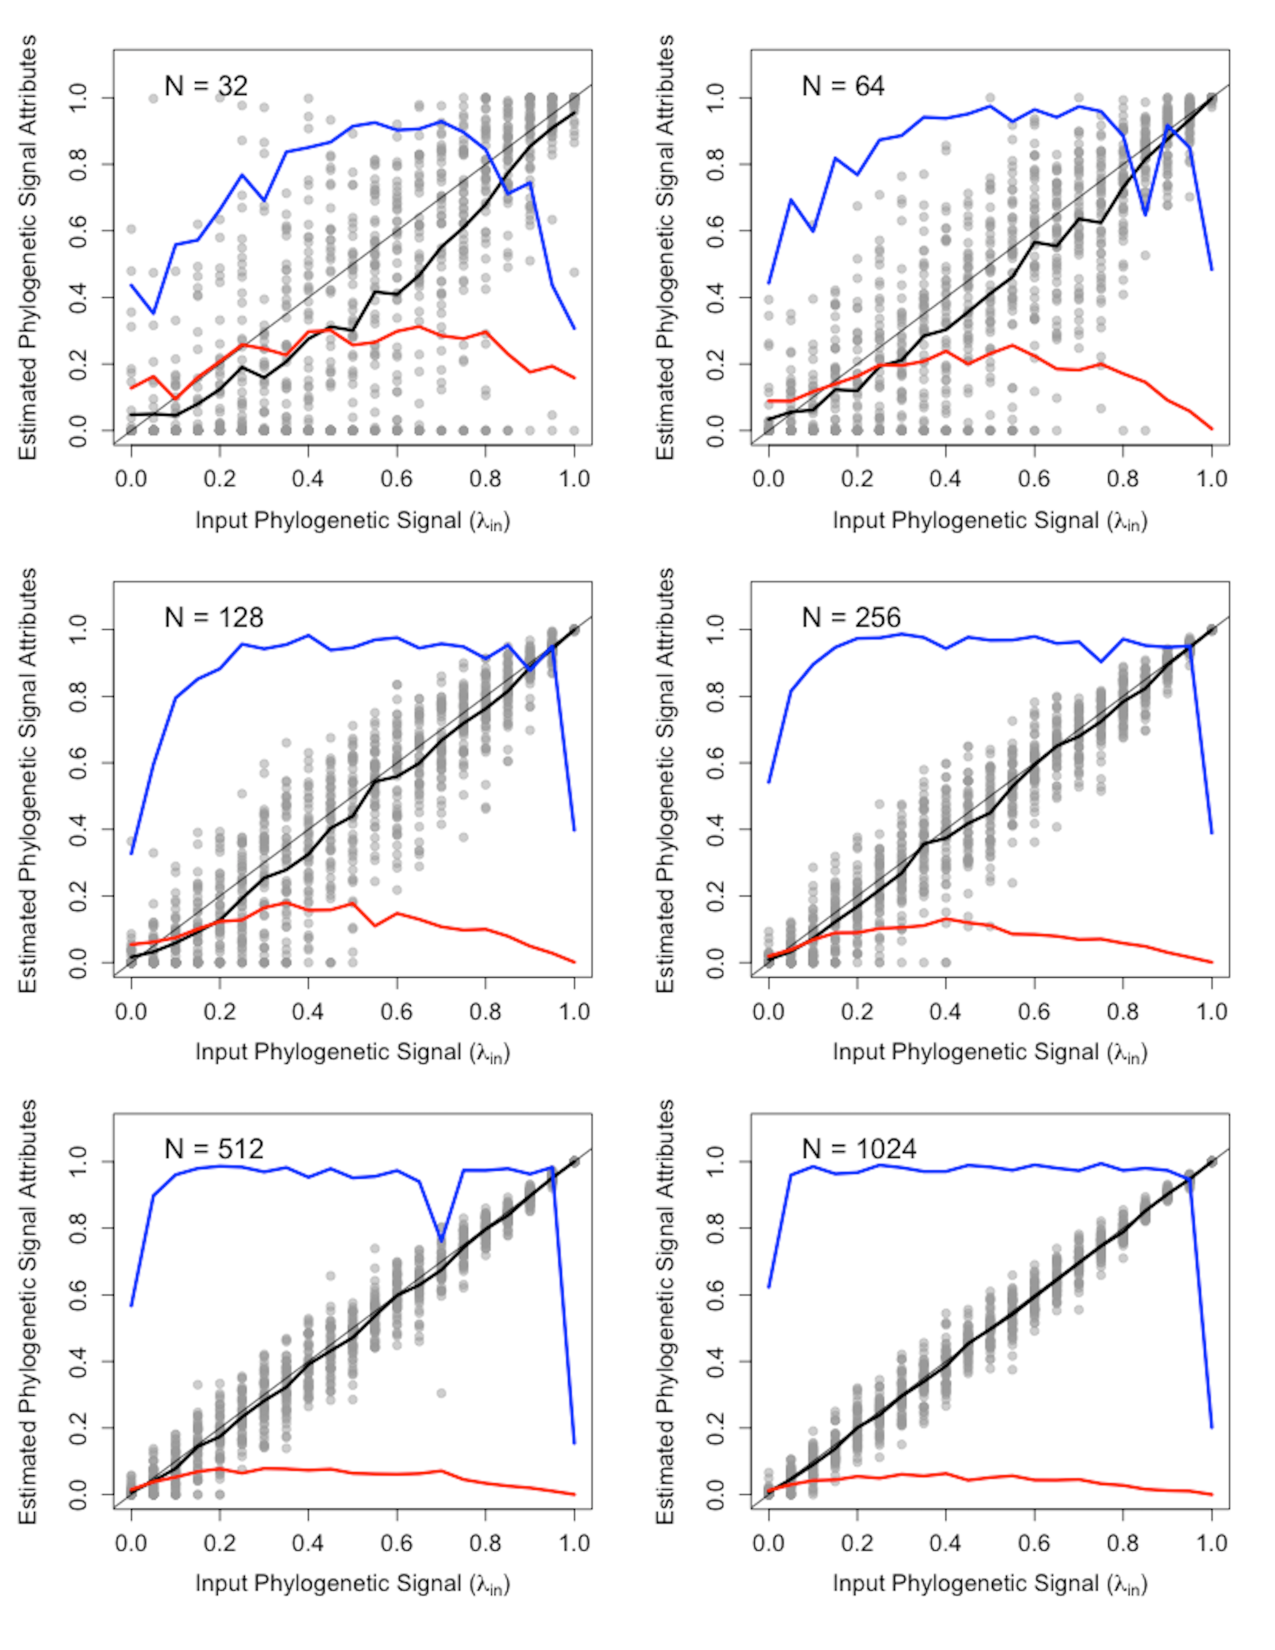
\includegraphics[width=1\linewidth]{Figs/fig.1} \caption{Response of Pagel's $\lambda$ to increasing strength of Brownian motion. Gray line signifies the 1:1 line where the input value matches the estimate $\hat\lambda$. At each input level, the dark black line represents the empirically derived expected value (mean) of $\hat\lambda$, the red line is the standard deviation of $\hat\lambda$, and the blue line is Shapiro Wilks statistic of $\hat\lambda$ ($W=1.0$ signifies normality, $W< 1.0$ represent skewed distributions). }\label{fig:unnamed-chunk-3}
\end{figure}

\begin{figure}
\includegraphics[width=1\linewidth]{Figs/fig.2} \caption{Response of Blomberg's $K$ to increasing strength of Brownian motion.  At each input level, the black line represents the empirically derived expected value (mean) of $K$, the red line is the standard deviation of $K$, and the blue line is Shapiro Wilks statistic of *K* ($W=1.0$ signifies normality, $W< 1.0$ represent skewed distributions).}\label{fig:unnamed-chunk-4}
\end{figure}

\begin{figure}
\includegraphics[width=1\linewidth]{Figs/fig.3} \caption{Response of effect sizes $Z_\lambda$ and $Z_K$ to increasing strength of Brownian motion.  Means from simulation runs are shown for comparative ease. Individual values from each simulation run are available in Supporting Information.}\label{fig:unnamed-chunk-5}
\end{figure}

\begin{figure}
\includegraphics[width=24.22in,height=0.75\textheight]{Figs/fig.4} \caption{Type I error rates and model misspecification for $\hat{Z}_{12}$. Type I error is found on the far-left of the plot ($\lambda = 0$). The black line signifies the average type I error and false discovery rates across simulations of different tree sizes.}\label{fig:unnamed-chunk-6}
\end{figure}

\begin{figure}
\includegraphics[width=0.9\linewidth]{Figs/fig.5} \caption{(A) Linear measures for relative body size, and regions of the body used to estimate surface area to volume (SA:V) ratios. (B) Permutation distributions of phylogenetic signal for SA:V and $\frac{BW}{SVL}$, with observed values shown as vertical bars. (C) Effect sizes ($Z_K$) for SA:V and $\frac{BW}{SVL}$, with their 95\% confidence intervals (CI not standardized by $\sqrt(n)$).}\label{fig:unnamed-chunk-7}
\end{figure}

\end{document}
